% fancytikzposter.tex, version 2.1
% Original template created by Elena Botoeva [botoeva@inf.unibz.it], June 2012
% 
% This file is distributed under the Creative Commons Attribution-NonCommercial 2.0
% Generic (CC BY-NC 2.0) license
% http://creativecommons.org/licenses/by-nc/2.0/ 
\documentclass{a0poster}
\usepackage[USenglish]{babel}% or british
\usepackage[T1]{fontenc}


\usepackage{wrapfig}
\usepackage{fancytikzposterM} 
\usepackage{multirow}
\usepackage{array}

% background picture
\usebackgroundtemplate{7}

\definecolor{myblue3}{HTML}{0C3E07}%main frames


\usepackage[margin=\margin cm, paperwidth=84.1cm, paperheight=118.9cm]{geometry}


\usepackage{cmbright}
%\usepackage[default]{cantarell}
%\usepackage{avant}
%\usepackage[math]{iwona}
\usepackage[math]{kurier}
\usepackage[T1]{fontenc}
\usepackage{tikz}

%%%%%%%%%%%%%%%%%%%%%%%%%%
%%% SET FONT SIZES %%%%%%%%%%%%%
%%%%%%%%%%%%%%%%%%%%%%%%%%
\renewcommand{\Huge}{\fontsize{64}{85}\selectfont} % Main title
\renewcommand{\huge}{\fontsize{44}{70}\selectfont} % Sub title
\renewcommand{\LARGE}{\fontsize{48}{48}\selectfont} % Box headers
\renewcommand{\Large}{\fontsize{42}{40}\selectfont} % Authors
\renewcommand{\normalsize}{\fontsize{40}{42}\selectfont} % Text in the boxes
\renewcommand{\footnotesize}{\fontsize{34}{42}\selectfont} % references
\renewcommand{\small}{\fontsize{24}{22}\selectfont}
\newcommand{\smallest}{\fontsize{18}{16}\selectfont}
%% add your packages here


%% Set the folder that contains the images
\graphicspath{ {./Lowres/} }


\title{How much are wild vertebrate populations evolving right now?\vspace{-0.2em}}
\author{{\LARGE{Timoth\'{e}e Bonnet} \& Loeske Kruuk}\\ \vspace{-20pt} \footnotesize Australian National University
\\
}

\begin{document}

%%%%% ---------- the background picture ---------- %%%%%
%% to change it modify the macro \BackgroundPicture
%\ClearShipoutPicture
%\AddToShipoutPicture{\BackgroundPicture}

\noindent % to have the picture right in the center

\begin{tikzpicture}
  \initializesizeandshifts
  % \setxshift{15}
  \setyshift{2.5} % uncomment this line to condense the boxes

  \newcommand{\volesize}{0.8cm}

  %% the title block, #1 - shift, the default value is (0,0), #2 - width, #3 - scale
  %% the alias of the title block is `title', so we can refer to its boundaries later
  \ifthenelse{\equal{\template}{1}}{ 
    \titleblock[(-0.7,0)]{48}{1}
			}{
    \titleblock[(-10,0)]{87}{1.5}
			}
			
\addlogo[east]{(10,0)}{8cm}{loeske}
\addlogo[west]{(-10,0)}{8cm}{tim}

\coordinate (aaa) at (currenty);

	\blocknodew[($(currenty)+(19.6,0)$)]{77}{\textsc{The big problem:} We do not know how much wild organisms are currently evolving!}
		{Fisher's fundamental theorem of natural selection states that \textbf{additive genetic variation in fitness measures evolution across all traits and all the genome}. That is just what we need{\color{colorone}{\**}}!
		Yet, there are few estimates in free-ranging populations, and most may be unreliable. Indeed, it is difficult to measure fitness, difficult to estimate genetic variance, statistical models tend not to fit the data, and it is unclear how to interpret estimates from generalized linear models. We assemble data from the monitoring of a dozen pedigreed populations, 
		}
	
%%%%%%%%%%%%%%%%%%%%%%%%%%%%%%%%%%%%%%%%%%%%%%%%%%%%%%%%%%%%%%%%%%%%%%%%%%%%%	
	\blocknodew[($(currenty)+(0,2)$)]{77}{\textsc{Theory:} How to estimate additive genetic variance in relative fitness ($V_A(\omega)$) ?}
	{	
	\hspace{-1cm}
		\begin{tabular}{p{0.30\textwidth} p{0.029\textwidth} p{0.30\textwidth} p{0.029\textwidth} p{0.30\textwidth}}
		
		\parbox{24cm}{ \hspace{2cm} {\textsc{How to model fitness?}\\
		
		  \centering  \begin{tabular}{c c}
		    \includegraphics[width=20cm]{Rgraph/figure/zidist-1.pdf}
		    \end{tabular}
		    
		    }
		     \footnotesize Zero-Inflated Over-Dispersed Poisson models tend to fit well lifetime fitness data. Quantitative genetic estimates may be more precise than with Gaussian or Poisson models.
		  }
		&

		&
		\parbox{24cm}{ \hspace{1cm} \textsc{How to estimate genetic variation?}\\
		
		   {\centering \begin{tabular}{c} 
		   \includegraphics[width=20cm]{Rgraph/figure/latentGmat-1.pdf}
		   \end{tabular}
		   
		   }
		   \footnotesize Quantitative genetic \textit{\textsc{animal models}} use relatedness matrix to estimate G-matrix for the zero-inflation and the over-dispersed Poisson processes on two latent scales (log and logit).
		  }
		&
		  
		&
		\parbox{24cm}{\textsc{How to convert estimates to $V_A(\omega)$}\\
		
		{\centering \begin{tabular}{c}
		  \includegraphics[width=20cm]{Rgraph/figure/DlambdaZI-1.pdf}
		\end{tabular}} 
				
		\footnotesize Monte-Carlo integration of latent breeding values to the scale of data. Back-transformation works: with simulations $V_A(\omega)$ equals the increase in population growth rate.
	      }
		\end{tabular}
		\vspace{-1cm}
	}%end block
%%%%%%%%%%%%%%%%%%%%%%%%%%%%%%%%%%%%%%%%%%%%%%%%%%%%%%%%%%%%%%%%%%%%%%%%%%%%%	
	\coordinate (tfirstcol) at (currenty);
	
 \coordinate (width) at ($(76.8,0) - (2.1,0)$);   
 %% the content of the block
          \draw let \p1=($(width)-(0,0)$) , \p2=($(0,\blocktitleheight cm)-(0,2.4cm)$)
          in node[draw, anchor=north, color=blocktitlefillcolor, text=blocktextcolor, 
          frame, rectanglesplittwo, rectangle split horizontal=false, 
          rectangle split part fill={blocktitlefillcolor, none}, %
          rectangle split empty part height= \y2 
          ]
          (box) at ($(currenty)+(0,2)$) {
            \nodepart{second}
            \begin{minipage}{\x1}
            \begin{center}
	      \vspace{22cm} % a very mesy trick to control box height...
            \end{center}
           \end{minipage}
          }; 

          %% the title of the block
          \node[frame, anchor=north west, text=blocktitletextcolor] at (box.north west)
          {\bf\LARGE \textsc{Emperical results:} };
          
          \node[anchor=north] (map) at ($(box.north)+(0,-3)$) {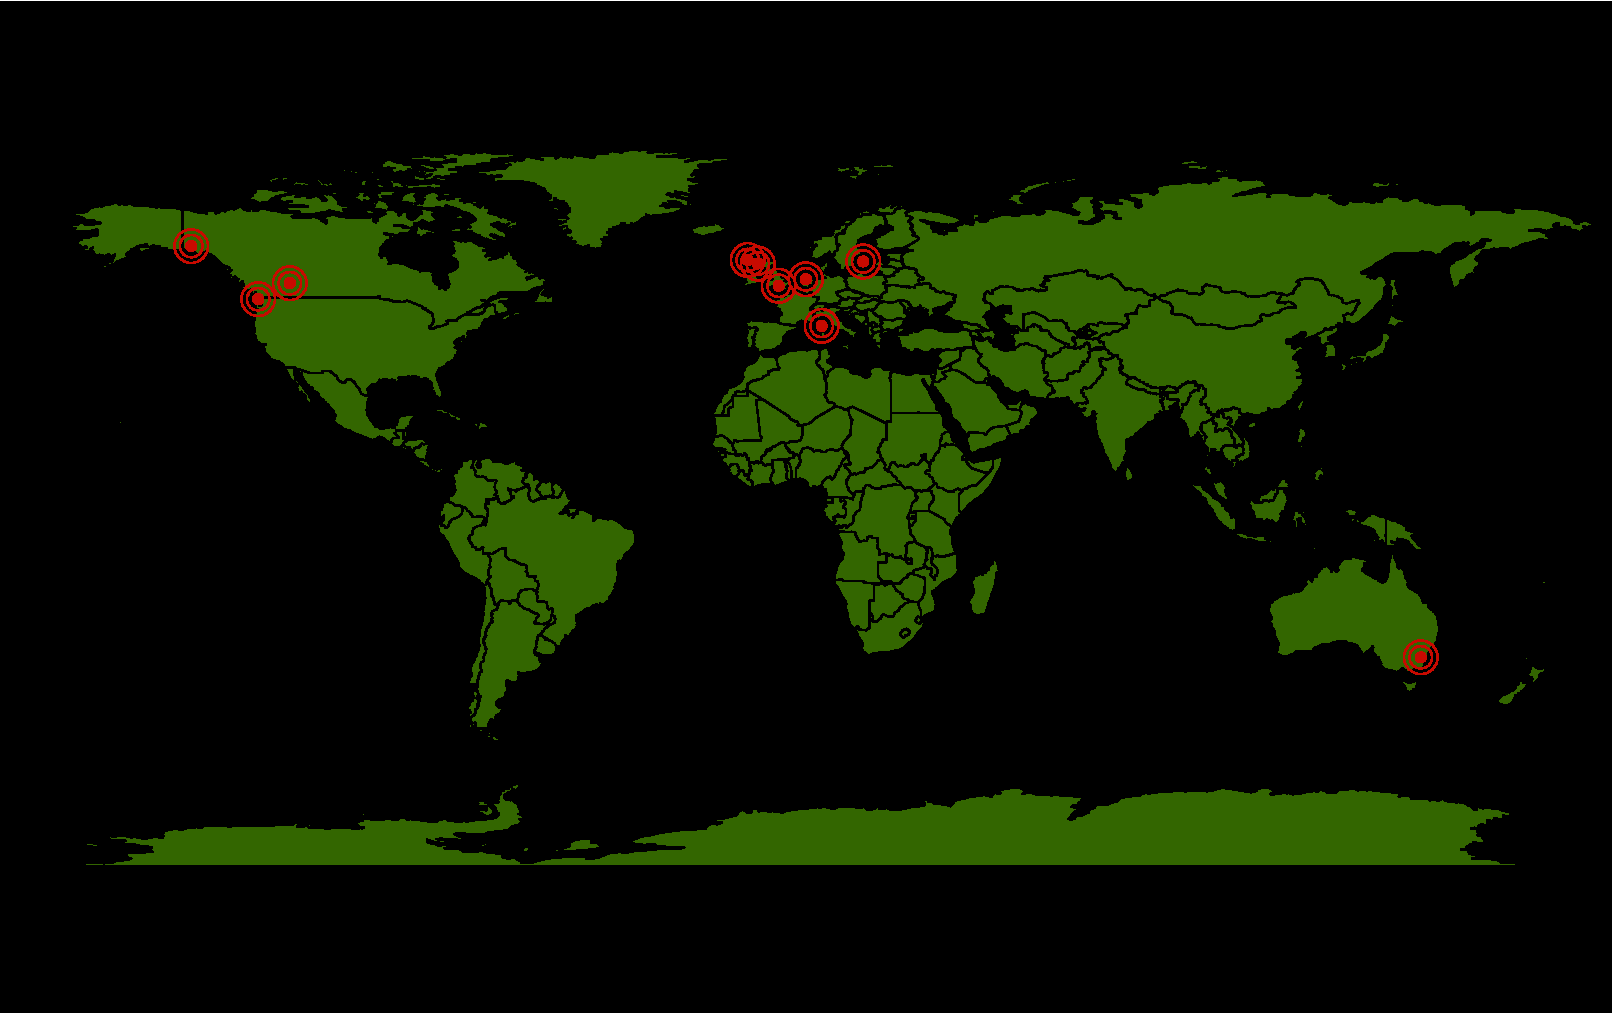
\includegraphics[width=20cm, trim=0cm 2.5cm 0cm 2.5cm, clip]{Rgraph/map.pdf}};

          \node[anchor=south west] (zih2) at (box.south west) {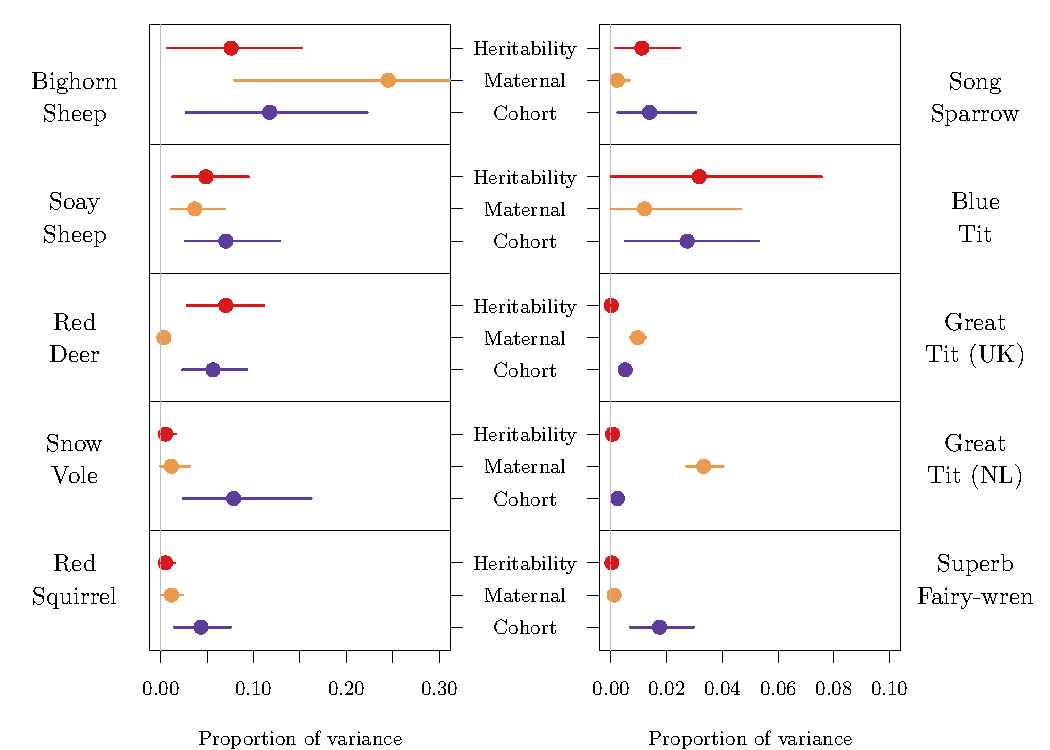
\includegraphics[width=20cm]{Rgraph/zih2.pdf}};
          %\node[anchor=north] (zih2com) at (zih2.south) {Heritabilities are small on the scale of the data\dots};
          
          \node[anchor=south east] (ziva) at (box.south east) {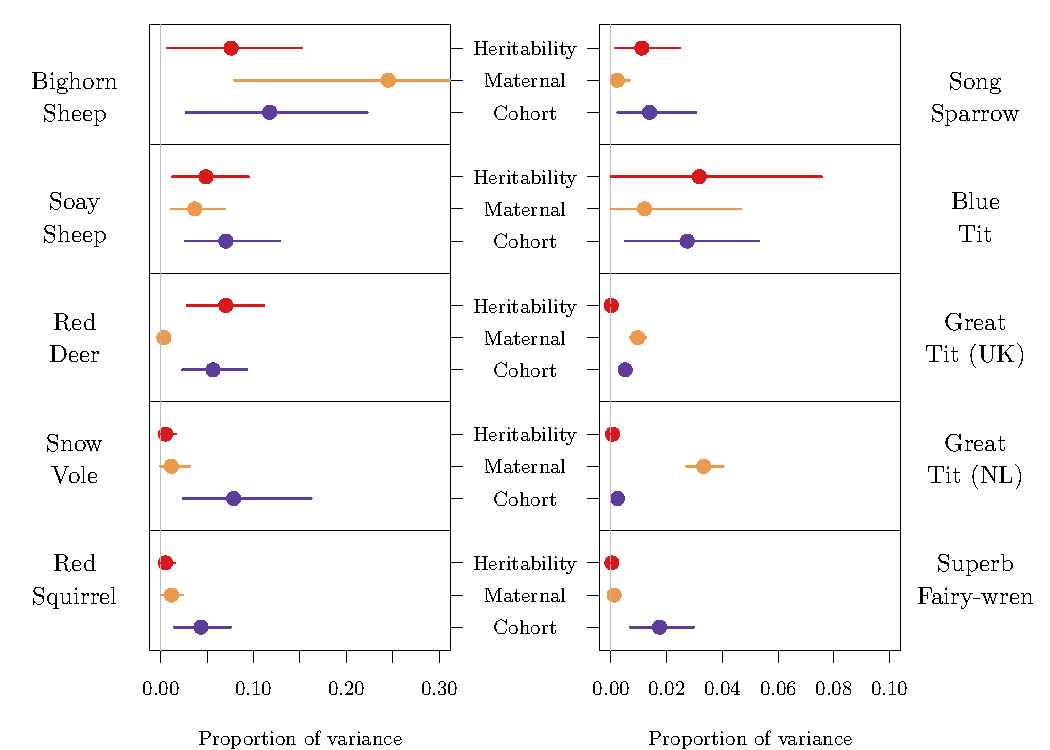
\includegraphics[width=20cm]{Rgraph/zih2.pdf}};
	  %\node[anchor=north] (zivacom) at (ziva.south) {\dots but that is irrelevant to the rate of evolution.};
                    
   \coordinate (currenty) at ($(box.south)-(yshift)$);
%%%%%%%%%%%%%%%%%%%%%%%%%%%%%%%%%%%%%%%%%%%%%%%%%%%%%

          
 %%%%%%%%%%%%%%%%%%%%%%%%%%%%%%%%%%%%%%%%%%%%%%%%%%%%%%%%%%%%%%%%%%%%%%%%%%%%%%%

    \node[anchor=north, rounded corners=15pt, fill=titledrawcolor] (qrw) at ($(currenty) + (-34,0)$) {
\includegraphics[width=8cm]{qrwebsite}};
    \node[anchor=north, rounded corners=15pt, fill=titledrawcolor] (qrgit) at ($(currenty) + (34,0)$) {
\includegraphics[width=8cm]{QRvawiswow}};
    \node[anchor=south] (web) at (qrw.north) {\textbf{\color{colorone!80!black}{Website}}};
    \node[anchor=north] (webadd) at ($(qrw.south)+(0,0.3)$) {\smallest{\color{colorone!80!black}{timotheenivalis.github.io}}};
    \node[anchor=south] (git) at (qrgit.north) {\textbf{\color{colorone!80!black}{R and \LaTeX code}}};
    \node[anchor=north] (gitadd) at ($(qrgit.south)+(0,0.3)$) {\smallest{\color{colorone!80!black}{github.com/timotheenivalis/VAWisWOW}}};

		
%%%%%%%%%%%%%%%%%%%%%%%%%%%%%%%%%%%%%%%%%%%%%		
   \Endblock{($(web.east)+(2,-4.5)$)}{57}{\hspace{25cm}\color{colorone}{\textsc{Co-authors:}}}{ 
   Michael Morrissey, Josephine Pemberton, Tim Clutton-Brock, Marco Festa-Bianchet, Andrew McAdam, Stan Boutin, Anne Charmantier,
C\'eline Teplistky, Christophe de Franceschi, Erik Postma, Glauco Camenisch,
Marcel Visser, Ben Sheldon, Simon Evans, Lars Gustafsson,
Jane Reid, Matthew Wolack \& Andrew Cockburn \\

{\color{colorone}{\**} Fisher's theorem relies on stringent assumptions, or alternatively on a specific meaning of evolution. In the absence of competition and gene-by-environment interactions, $V_A(\omega)$ is the increase in expected population growth rate. This clean link between evolution and demography probably doesn't apply (for long) in nature.}
  }
	
\end{tikzpicture}
  \end{document}
